\subsection{Visualization}
\begin{figure*}
    \centering
    \includegraphics[width=1\textwidth]{all_embeddings_subplot_copy.png}
    \caption{Visualizations of datasets with known hierarchical structure; (d) and (s) correspond to generated deep and shallow hierarchies, respectively. Multiclass noise in generated data is depicted in gray.}
    \label{fig:panel-fig}
\end{figure*}
Visualizations of text embeddings colored by top-level categories appear in Figure \ref{fig:panel-fig}. The generated hierarchies with 25\% noise are visualized. PHATE and PCA are better able to separate the noise class as compared with t-SNE and UMAP, but PHATE better preserves noise semantics by its centralized location, indicating a relation with multiple classes. PCA and t-SNE plots are globally quite similar, but t-SNE provides more class discriminability. PHATE, by contrast, displays top-level categories as extremal points of the embedding and provides cleaner class separation than PCA and t-SNE. UMAP collapses most of the information onto a single dimension in some cases and in others bears similarity to PHATE although compressing points and, in some cases, shattering the global structure. Additional visualizations with default parameter settings for UMAP and PHATE are provided in the appendices in Figure \ref{fig:default-visuals}.

The trajectory of topics and themes in the visualizations can be analyzed in several different ways. We visualize how the sub-themes within the Ecosystems data transition between the two themes of "Economic Impact Metrics" and "Social Conflict Intensity" (Figure \ref{fig:ecosystems-trajectory}). Similarly with the Fisheries data, we use the specific concepts to determine how some of the sub-themes mapped between the categories of "Offshore Energy Infrastructure Development," "Marine Environmental Quality," and "Fish Population Metrics" (Figure \ref{fig:fisheries-trajectory}). We, furthermore, curate semantic trajectories in the Web of Science embedding on the basis of keywords associated to each data point as provided in the dataset (Figure \ref{fig:WoS-trajectory}). Lastly, we use the information at the docket level for the EPA data to determine thematic changes over space (Figure \ref{fig:epa-trajectory}). 

\begin{figure*}
    \centering 
\begin{subfigure}{0.48\textwidth}
    \centering
    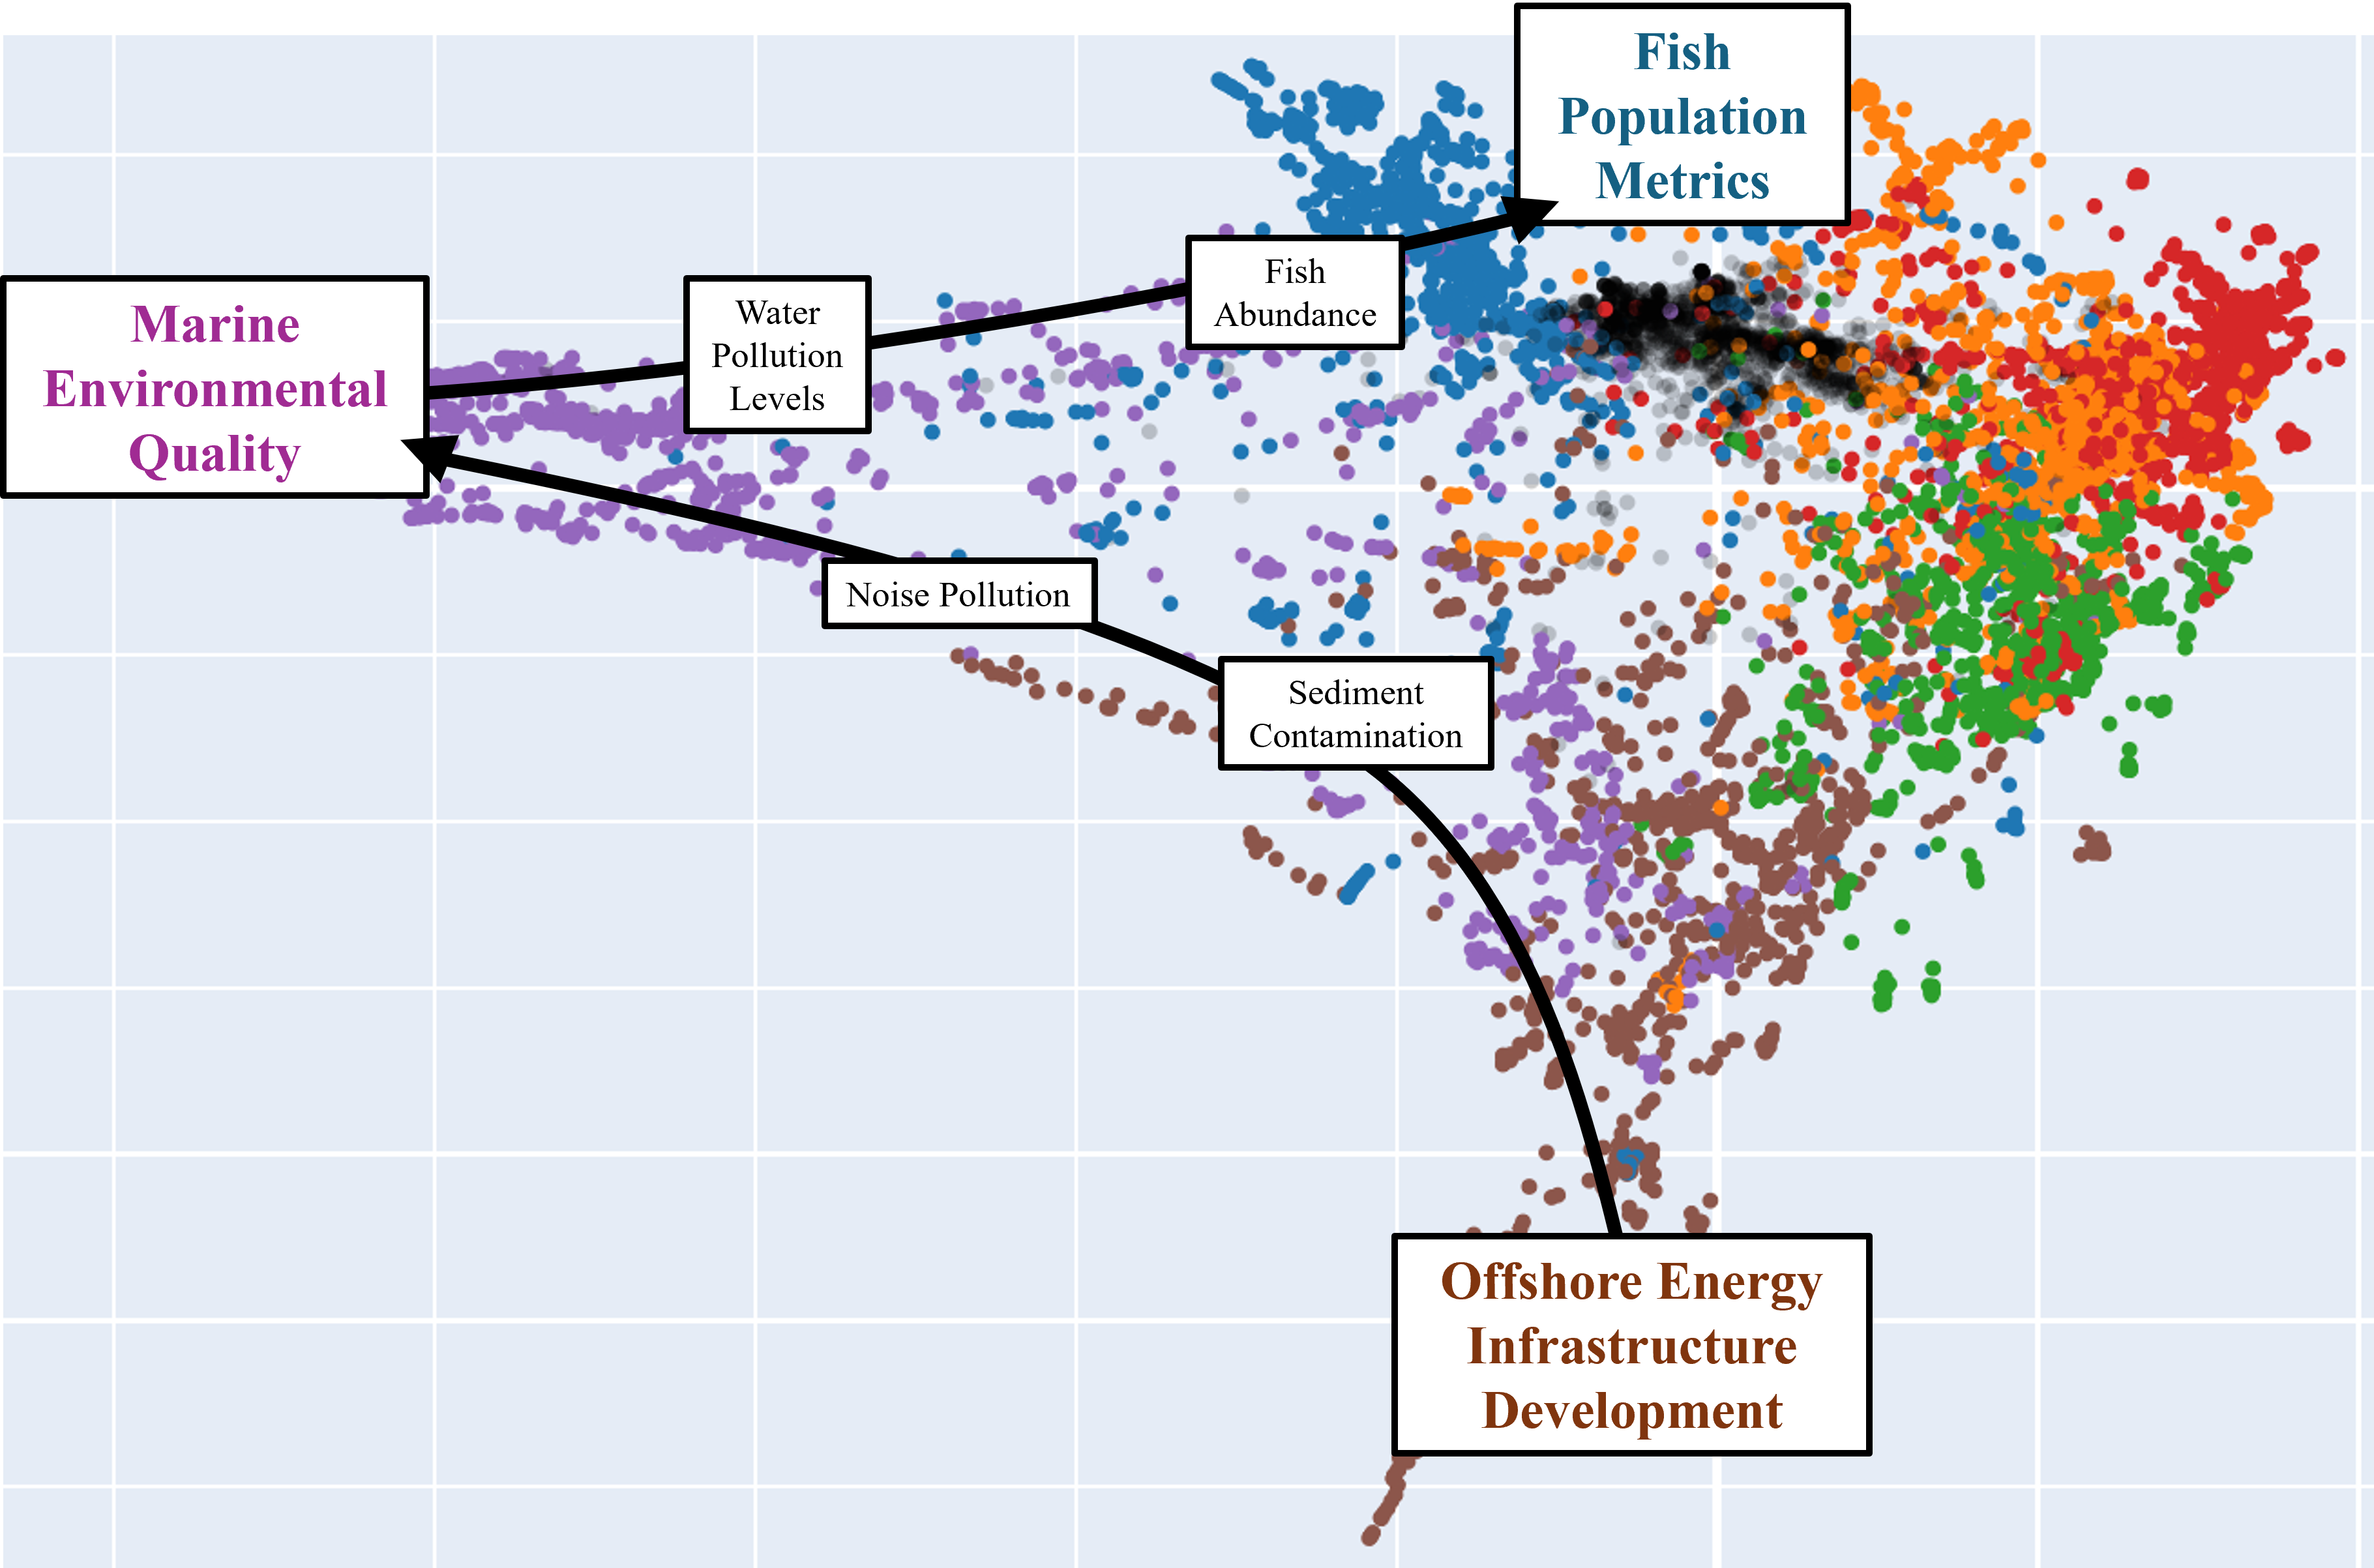
\includegraphics[width=\linewidth]{fisheries_trajectory.png}
    \caption{Trajectories in deep fisheries hierarchy}
    \label{fig:fisheries-trajectory}
\end{subfigure}
\begin{subfigure}{0.48\textwidth}
    \centering
    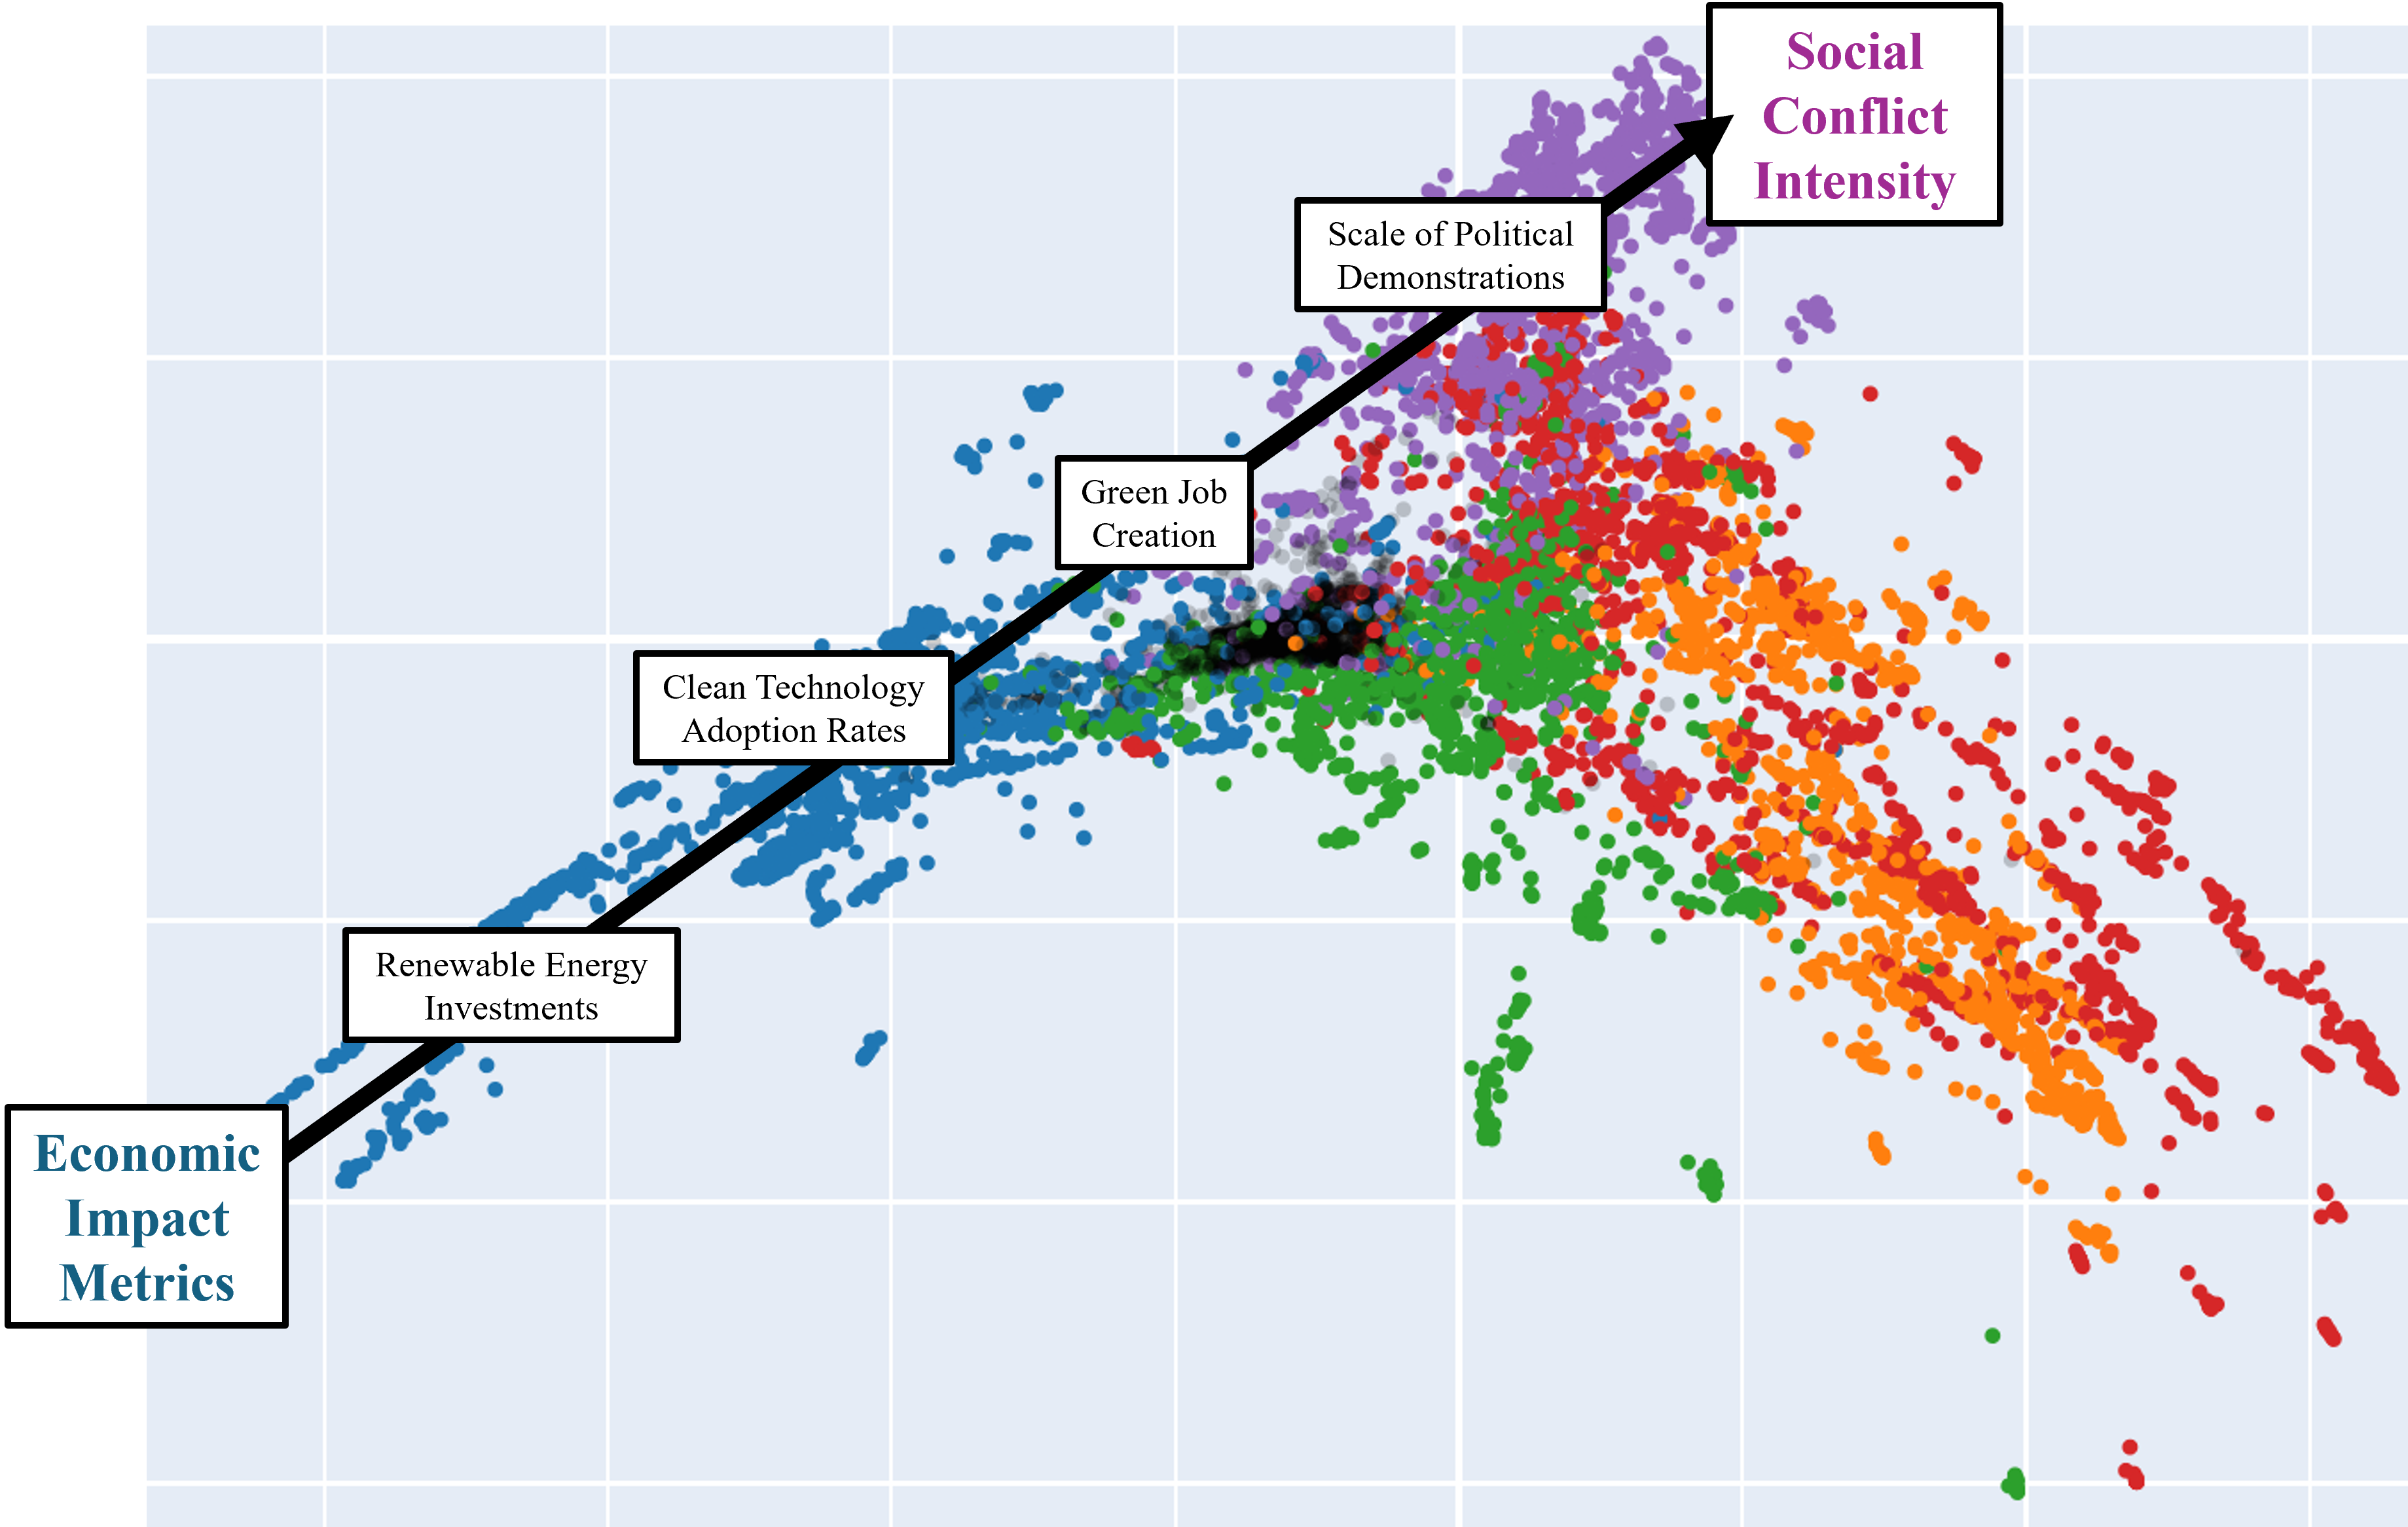
\includegraphics[width=\linewidth]{ecosystems_trajectory.png}
    \caption{Trajectories in deep ecosystems hierarchy}
    \label{fig:ecosystems-trajectory}
\end{subfigure}
\caption{"Narrative arc" trajectories in PHATE embedding space}
\label{fig:hierachy_trajectories}
\end{figure*}

\begin{figure*}
    \centering
    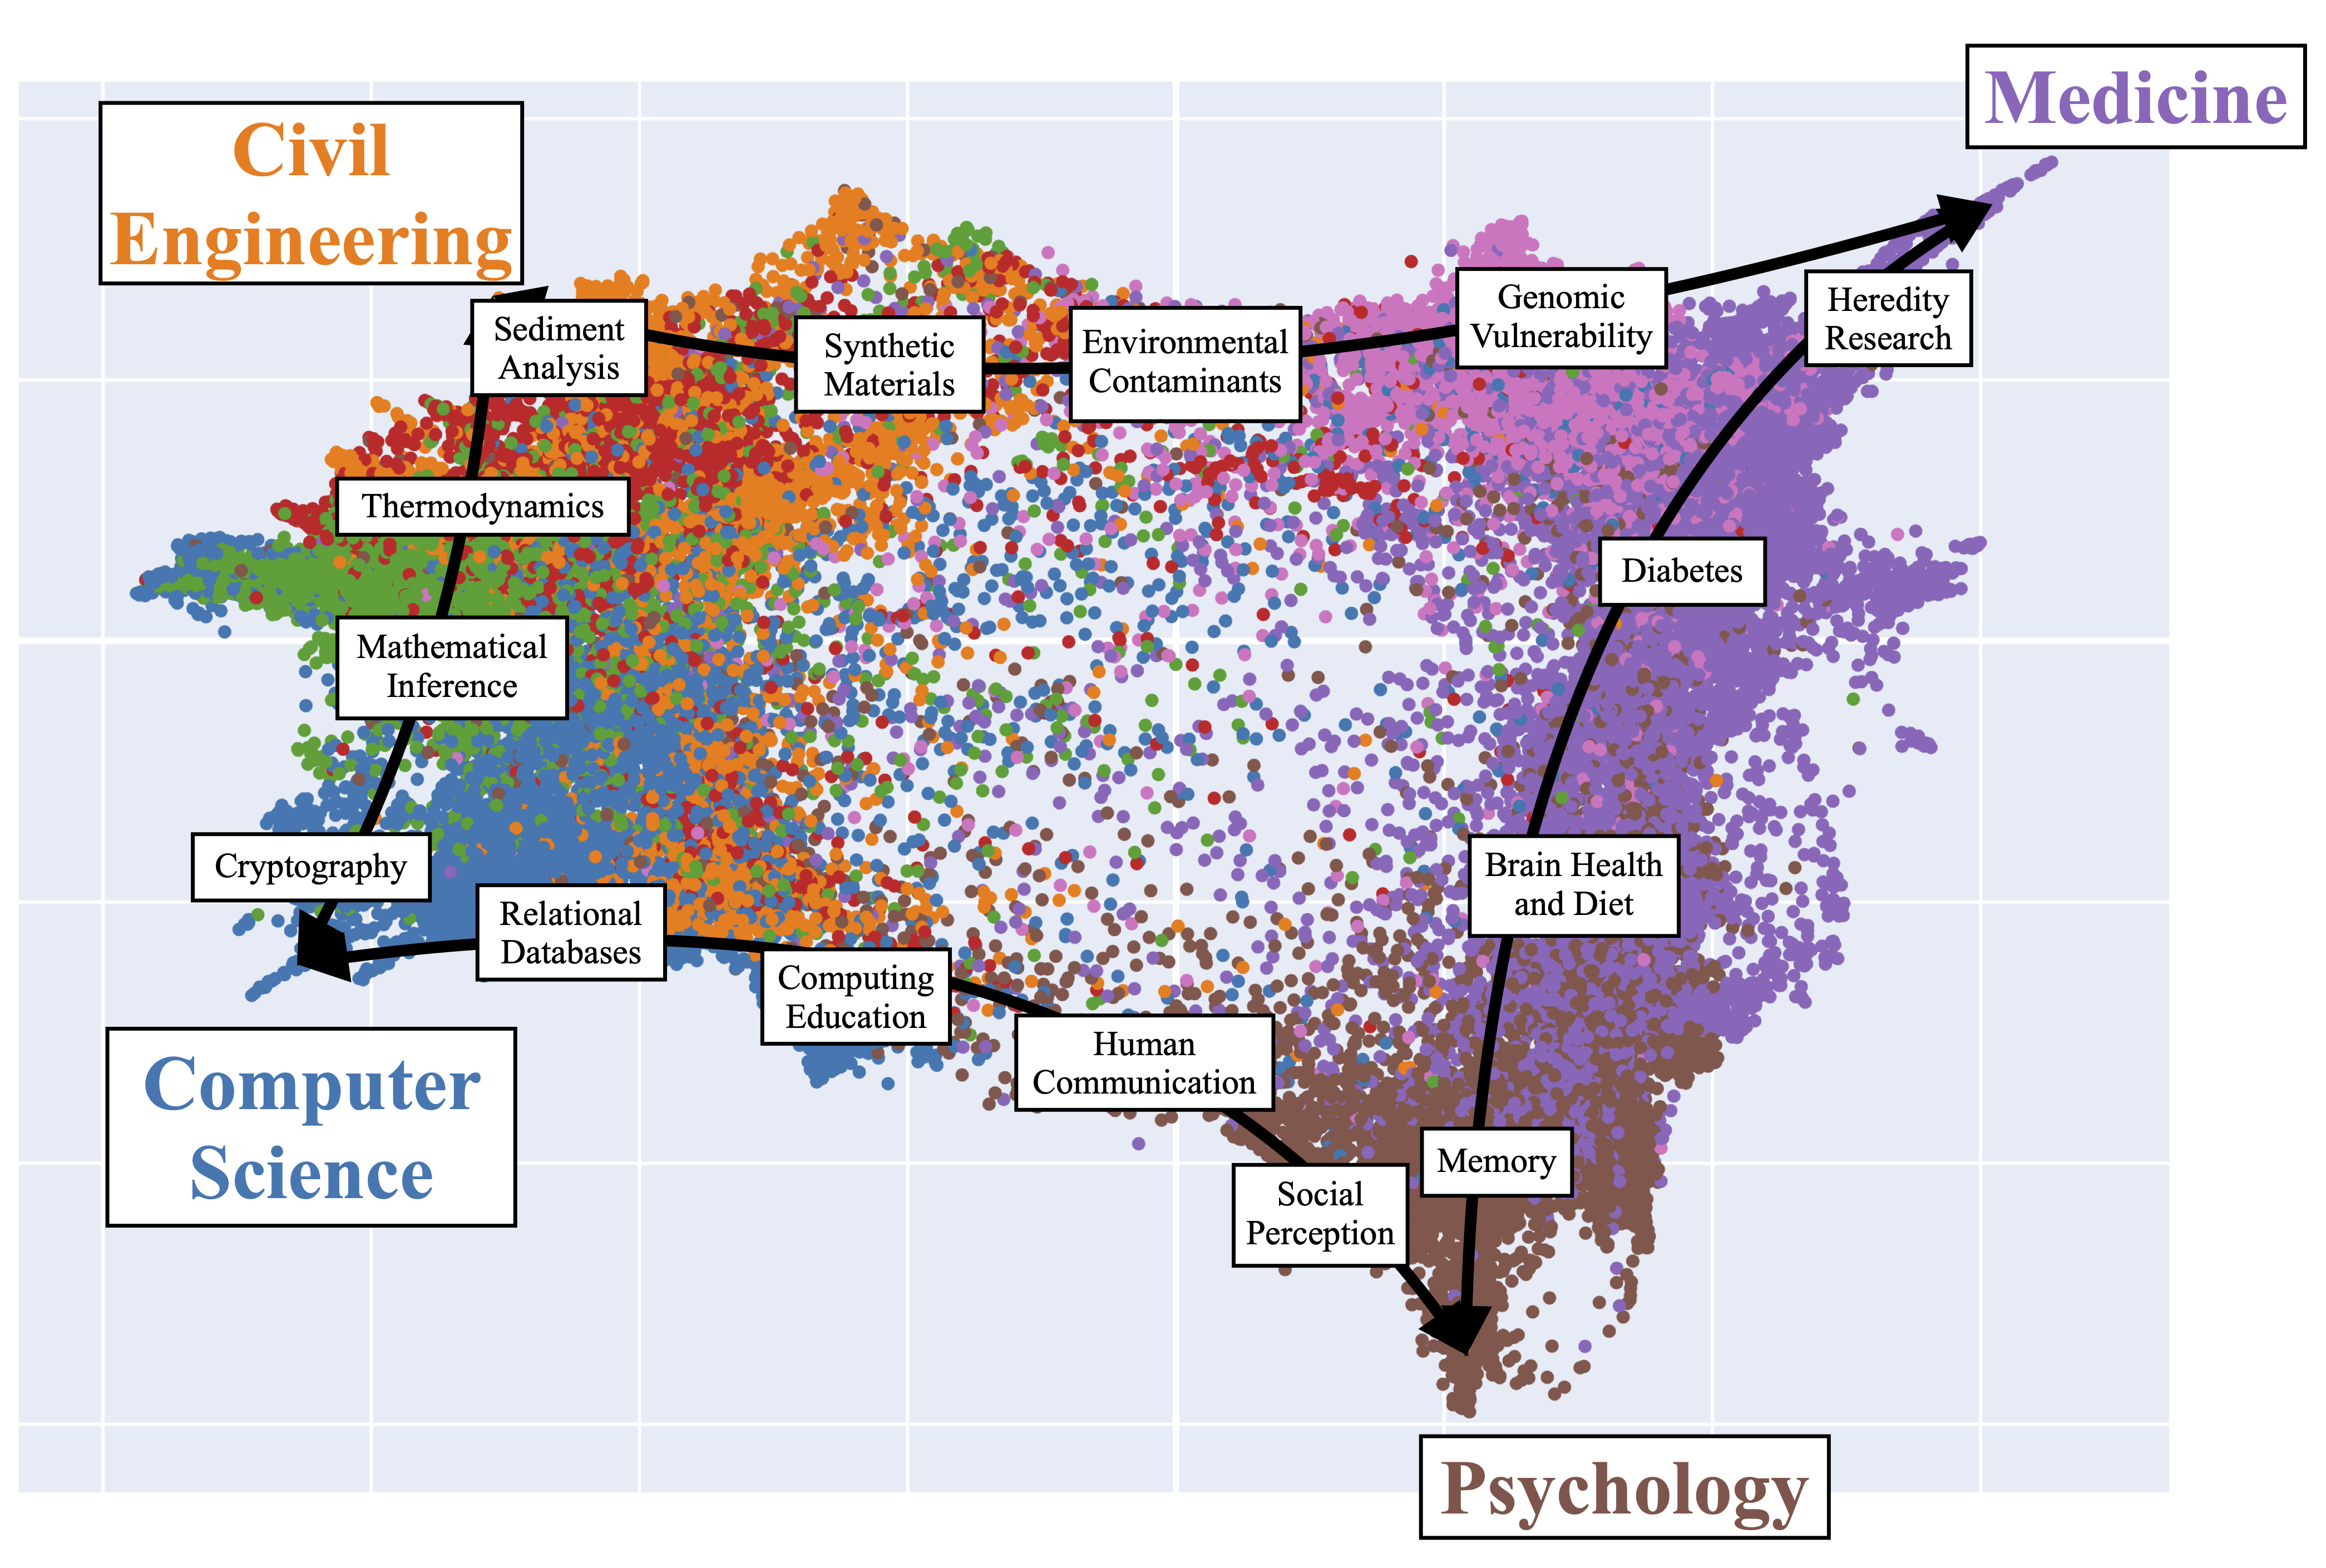
\includegraphics[width=1\linewidth]{phate_WOS.png}
    \caption{"Narrative arc" trajectories in PHATE embedding space of Web of Science}
    \label{fig:WoS-trajectory}
\end{figure*}  

\begin{figure}
    \centering
    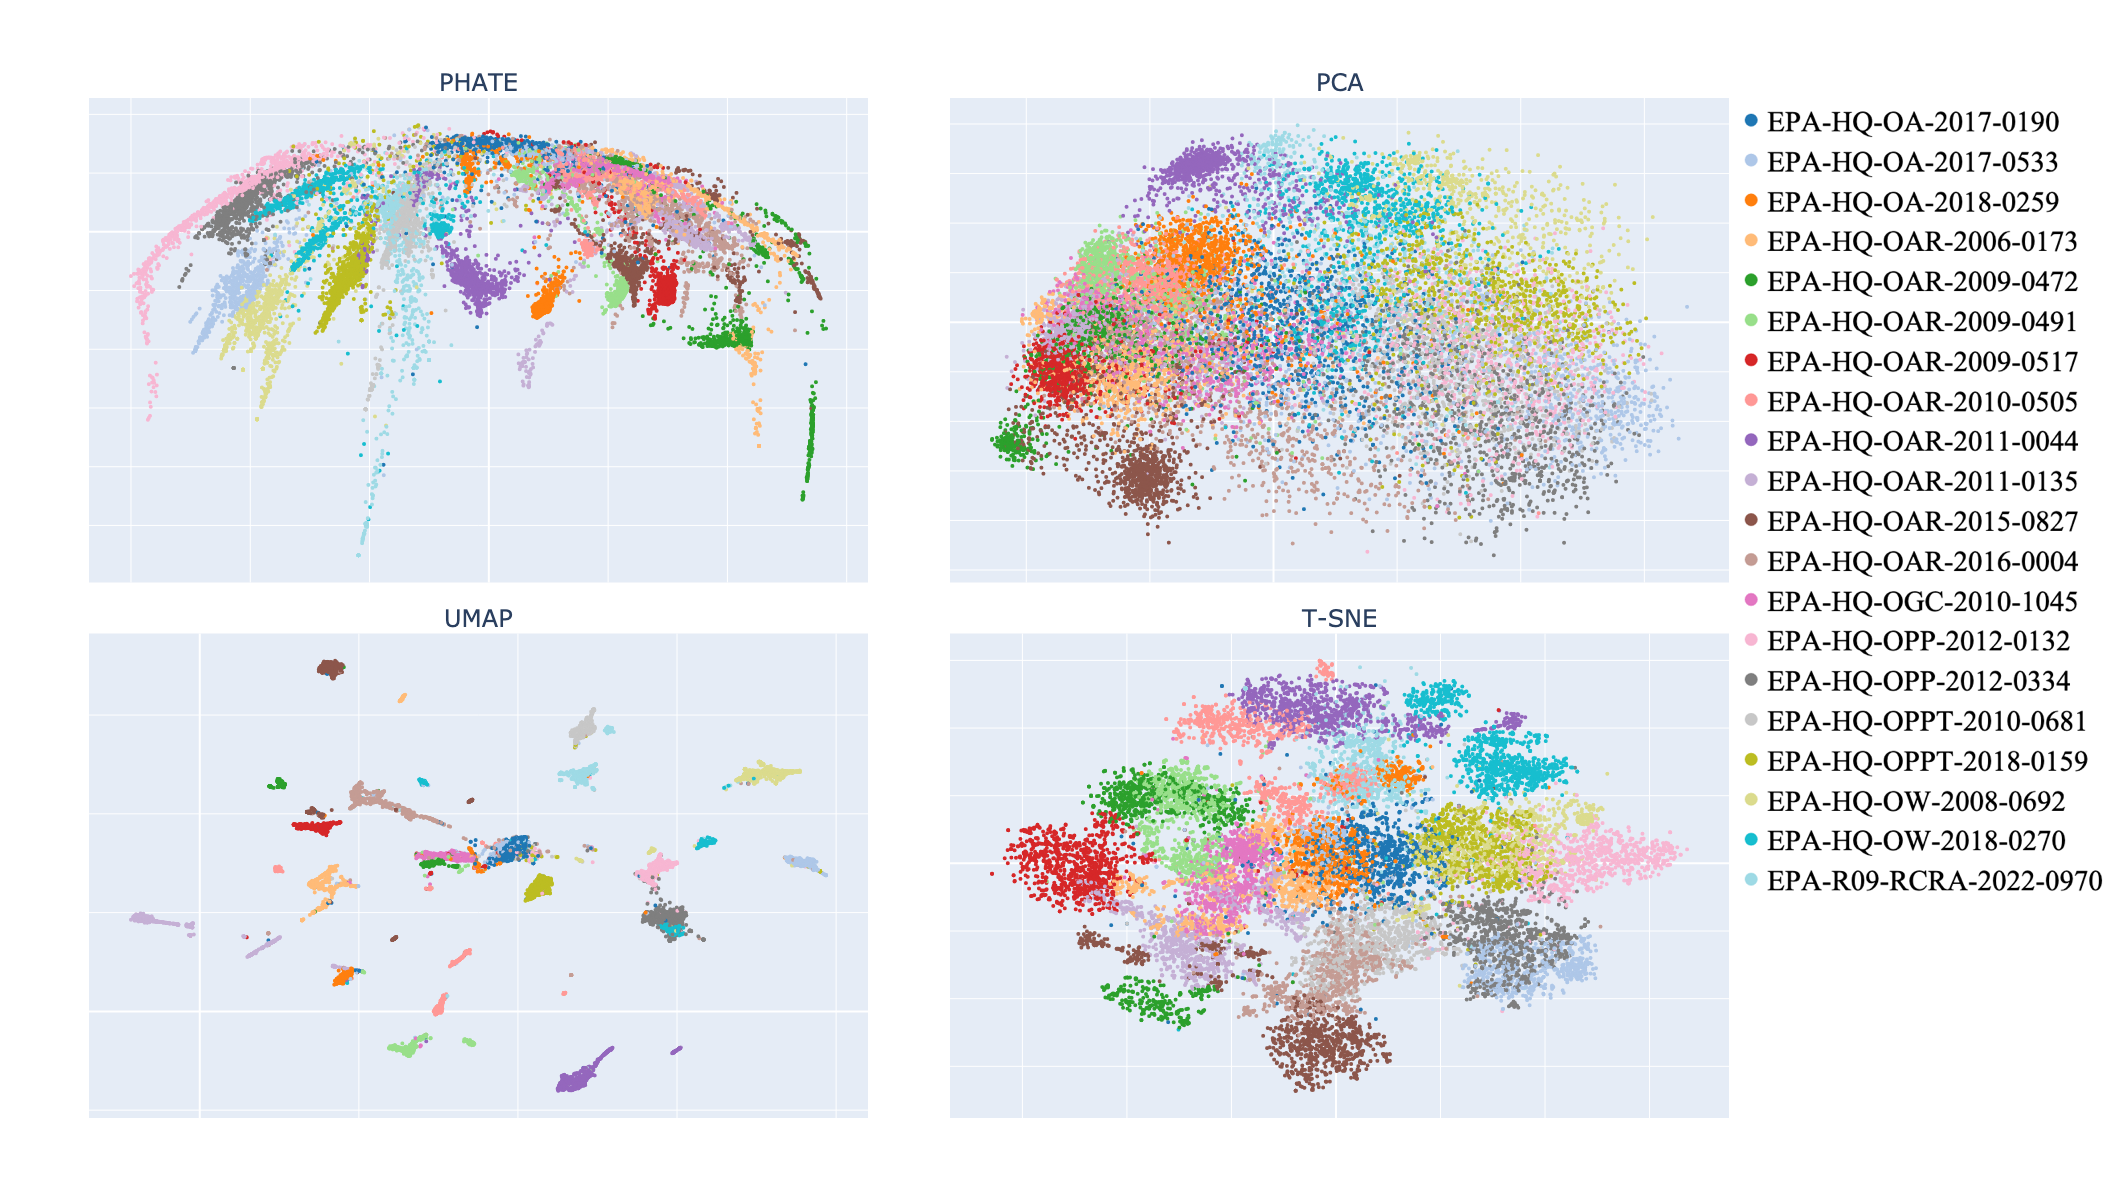
\includegraphics[width=1\linewidth]{epa_fig.png}
    \caption{Visualizations of head-tail embeddings of EPA comments colored by docket}
    \label{fig:epa-fig}
\end{figure}

\begin{figure}
    \centering
    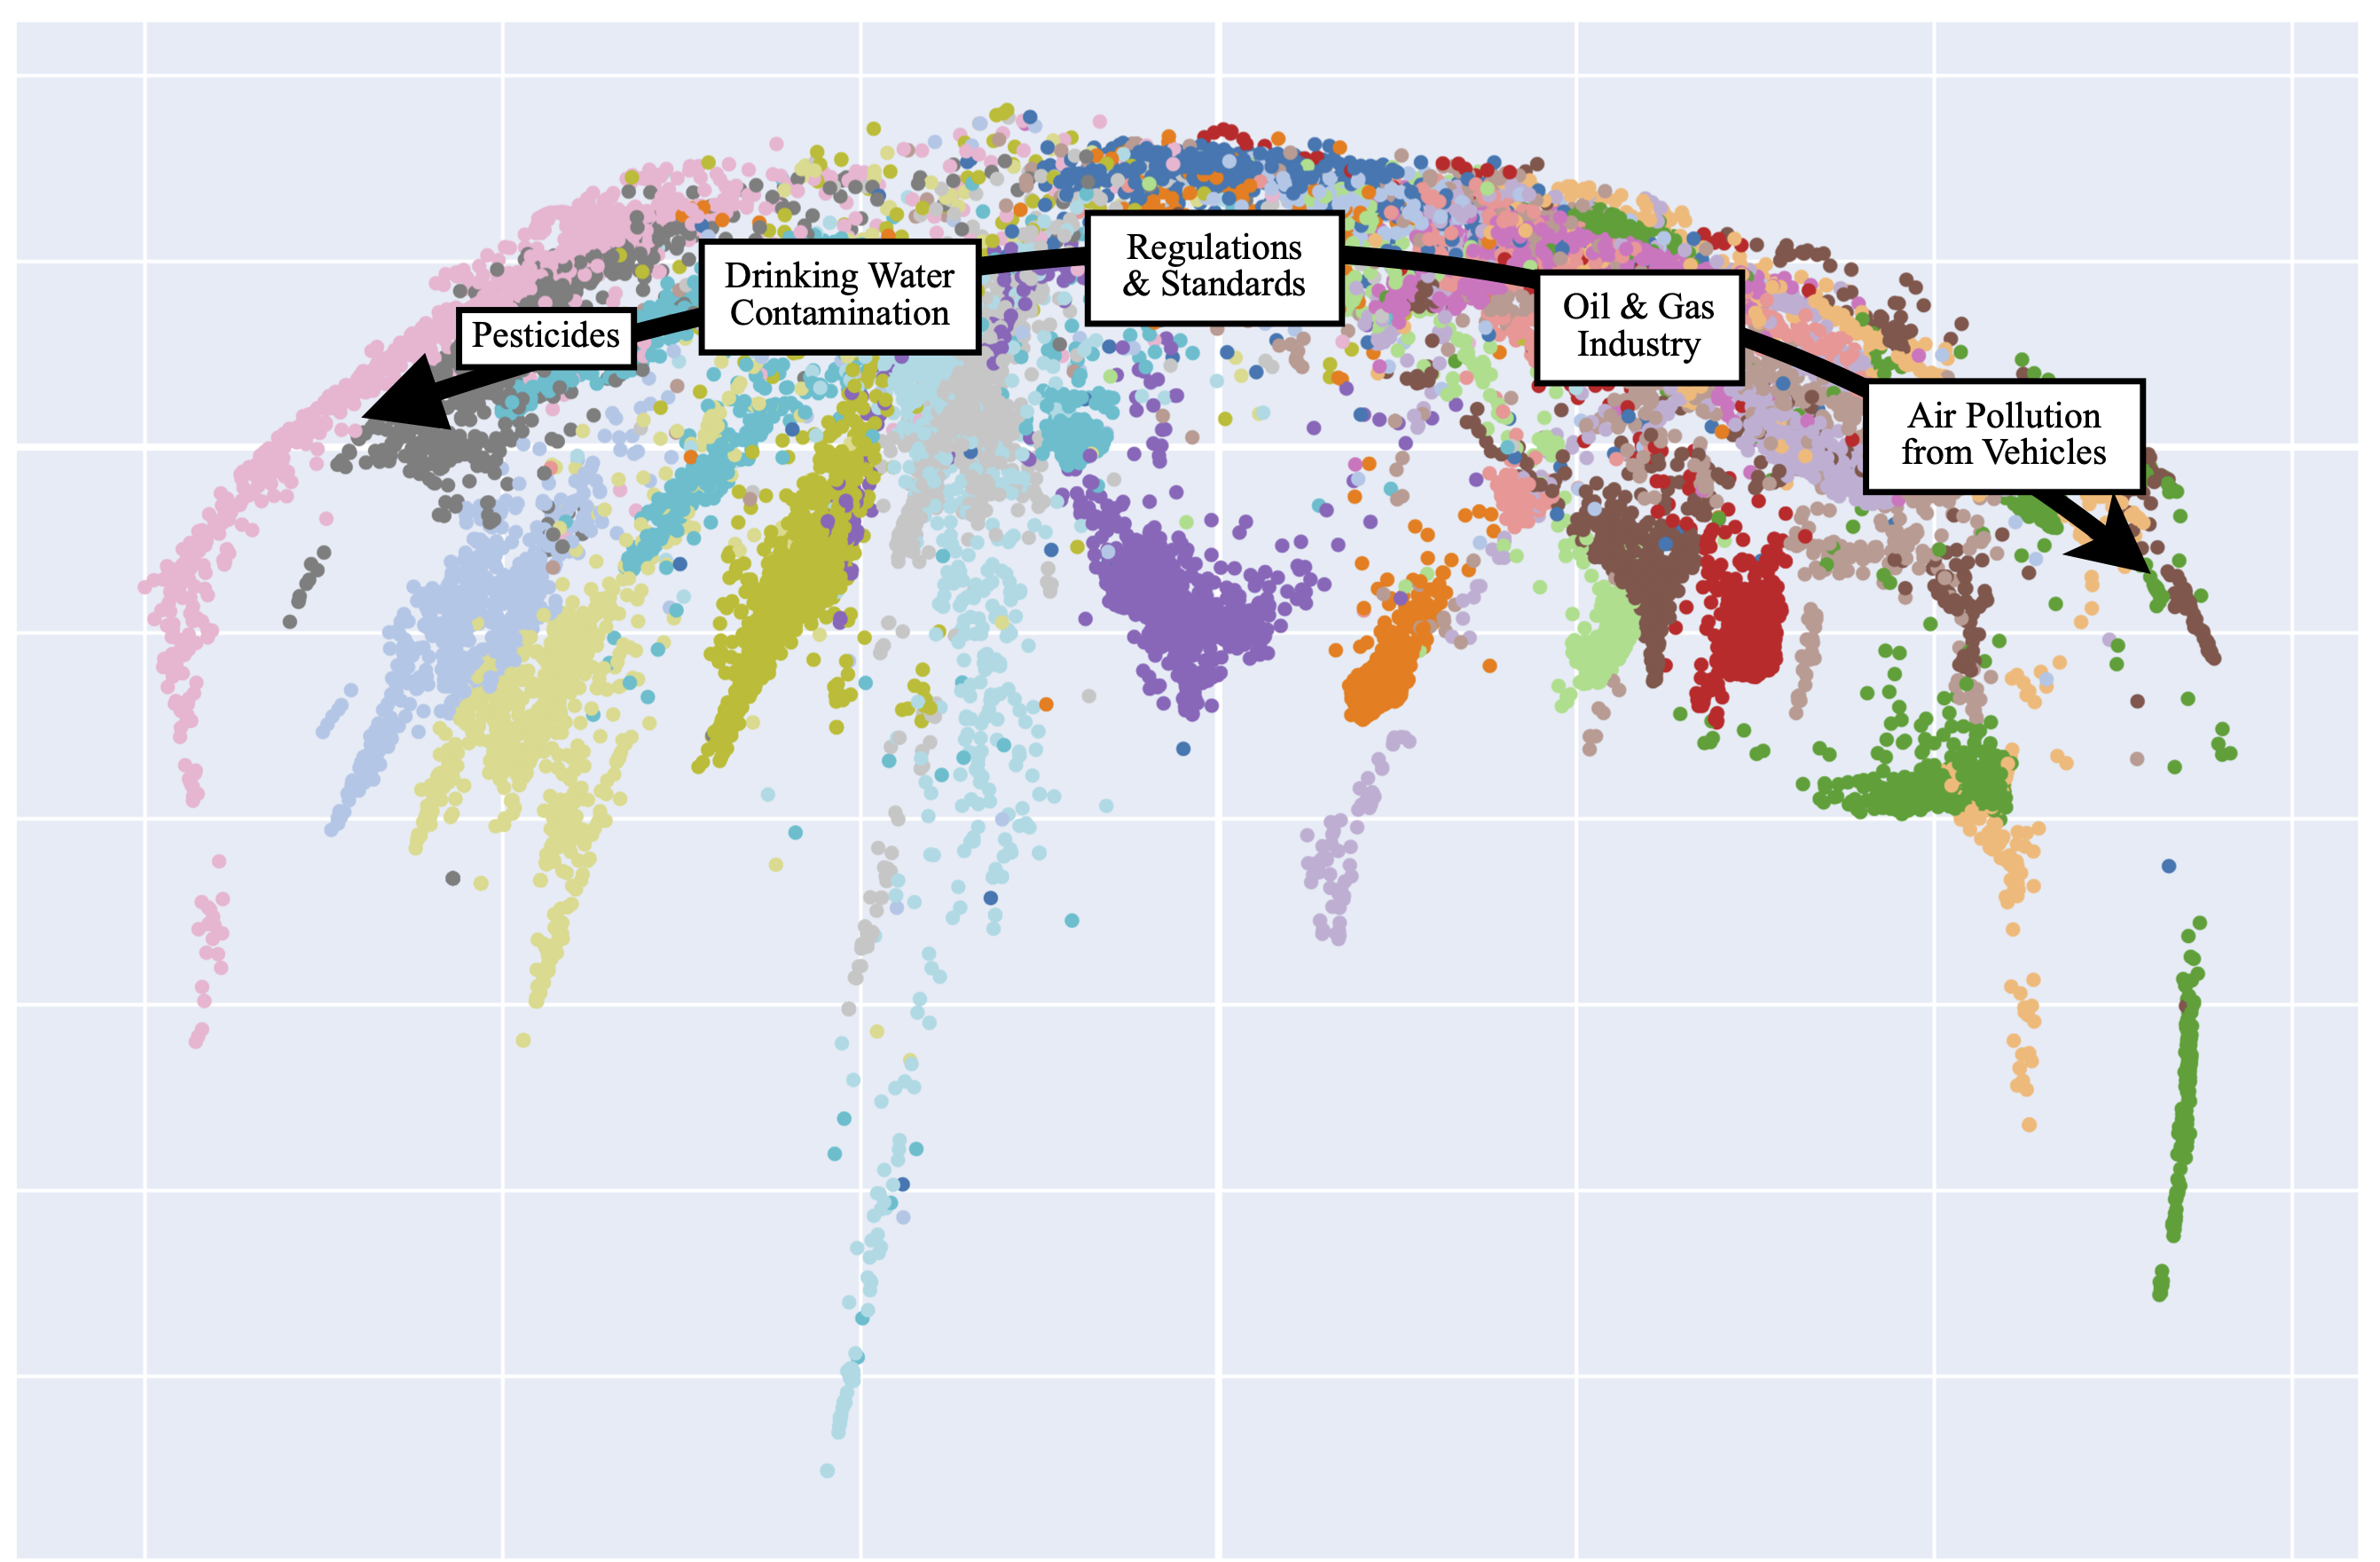
\includegraphics[width=1\linewidth]{epa_trajectory.png}
    \caption{"Narrative arc" trajectories in PHATE embedding space of EPA comments}
    \label{fig:epa-trajectory}
\end{figure}  

The visualization of PHATE compared to PCA, t-SNE and UMAP colored by the top 20 dockets is shown in Figure \ref{fig:epa-fig}. While PCA produces a dense and overlapping projection with limited visible structure, and t-SNE and UMAP highlight isolated clusters with distorted global relationships, PHATE preserves both local and global geometry using branching structures which suggest underlying transitions in comment themes across EPA dockets.
\FloatBarrier
\subsection{Dimensionality Reduction Evaluation}

Across all datasets, including both synthetic benchmarks and real-world datasets such as arXiv and RCV1, trustworthiness and continuity values are nearly identical across all dimensionality reduction methods, with values consistently around 0.5. This indicates that all methods preserve local neighborhood structure to a similar extent, and that performance is close to a random baseline, suggesting limited preservation of local neighborhood relationships when projecting high-dimensional embeddings to two dimensions.

Shepard diagrams show significant deviation from the diagonal across all methods, indicating that global distances are not well preserved. This suggests that dimensionality reduction introduces non-linear distortion, where distances are compressed in some regions and expanded in others.

Spearman rank correlation and DEMaP metrics further confirm that distance relationships between high-dimensional and low-dimensional spaces are only weakly preserved. Values are generally close to zero, indicating limited global structure preservation.

We observe that shallow hierarchical datasets (depth3) consistently achieve higher DEMaP and Spearman scores than deeper hierarchies (depth5), suggesting that simpler structures are easier to preserve in low-dimensional space.

Across methods, PHATE tends to achieve slightly higher DEMaP and Spearman values in some datasets, indicating improved preservation of manifold structure, although the differences are marginal. However, no single method consistently outperforms the others across all datasets.

These results highlight that commonly used dimensionality reduction methods exhibit similar trade-offs between local and global structure preservation when applied to high-dimensional text embeddings.
\subsection{Hierarchical clustering}
A summary of the performance of each method on the hierarchical clustering task appears in Table \ref{tab:pivot_table}. The reported values are the means over all cluster levels of the medians over all parameters for each method. PHATE and UMAP with agglomerative clustering each achieve the best or second-best performance on five of seven datasets. HDBSCAN consistently performs poorly on average as compared to diffusion condensation and agglomerative, regardless of dimensionality reduction method.  

\input{ari_table}


A more detailed presentation of the clustering results on the generated datasets appears in Figure \ref{fig:ARI-combined}. Reported values are means across datasets of medians at each cluster level for each method. While UMAP and PHATE coupled with HDBSCAN perform well at finer scales, these methods coupled with aggolomerative perform best at coarser scales. PHATE with diffusion condensation performs comparably to PCA with agglomerative, while slightly outperforming it on the deep hierarchies.

% A PHATE comparison of ground truth, top-level hierarchy labels, and those identified by diffusion condensation appears in [FIG]. Diffusion condensation differentiates clusters well, especially the noise class, with exceptions within class overlaps and notably the gold standard orange class. 

\begin{figure*}[htbp]
    \centering
    \begin{minipage}[t]{0.7\linewidth}
        \centering
        \begin{subfigure}[t]{0.49\linewidth}
            \centering
            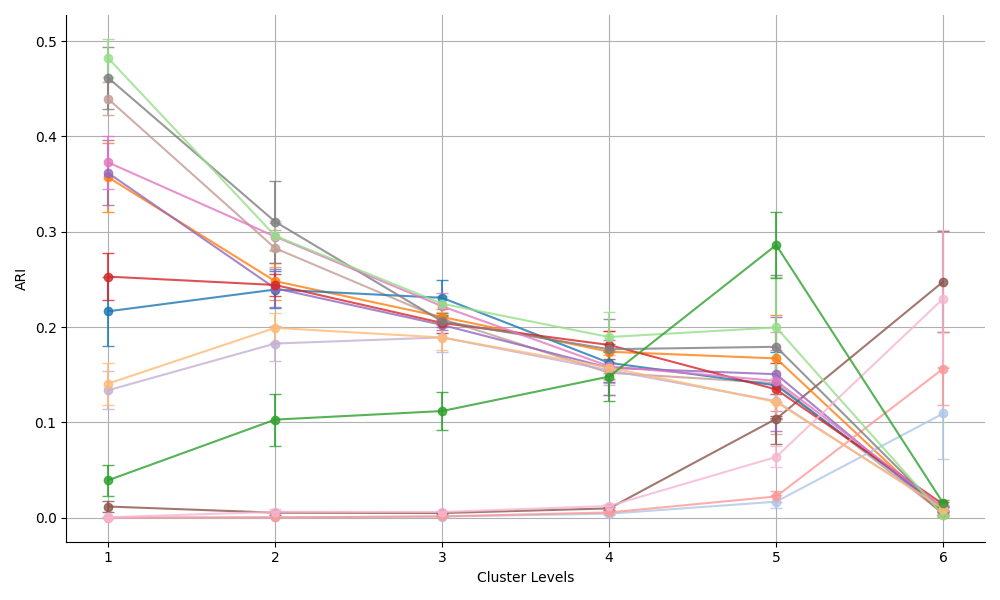
\includegraphics[width=\linewidth]{ARI_plot_None_hierarchy_t1.0_maxsub3_depth5_synonymsNone_noiseNone_random.png}
            \caption*{Deep datasets}
        \end{subfigure}
        \hfill
        \begin{subfigure}[t]{0.49\linewidth}
            \centering
            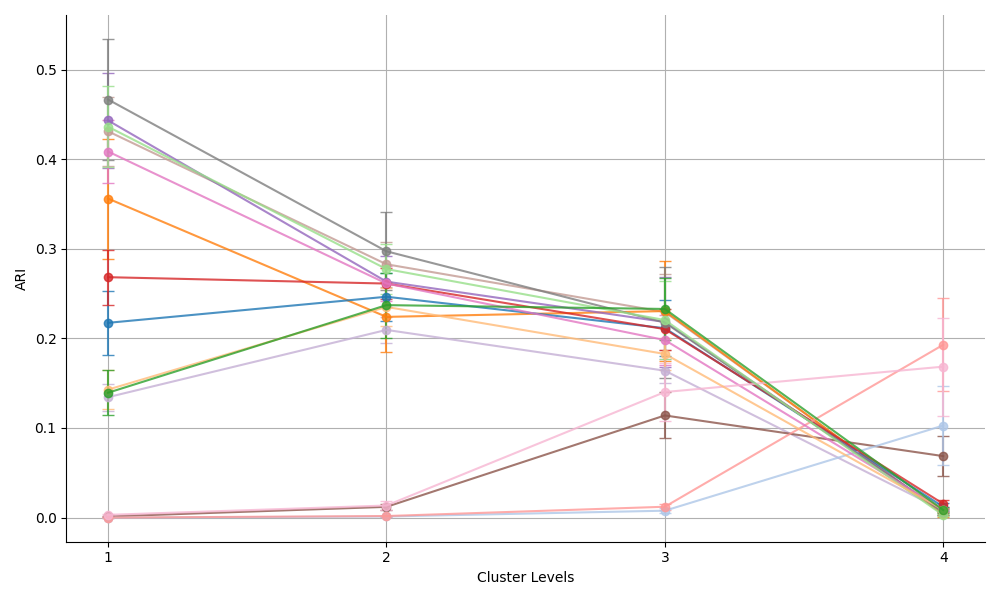
\includegraphics[width=\linewidth]{ARI_plot_None_hierarchy_t1.0_maxsub5_depth3_synonymsNone_noiseNone_random.png}
            \caption*{Shallow datasets}
        \end{subfigure}
    \end{minipage}
    \hfill
    \begin{minipage}[t]{0.25\linewidth}
        \centering
        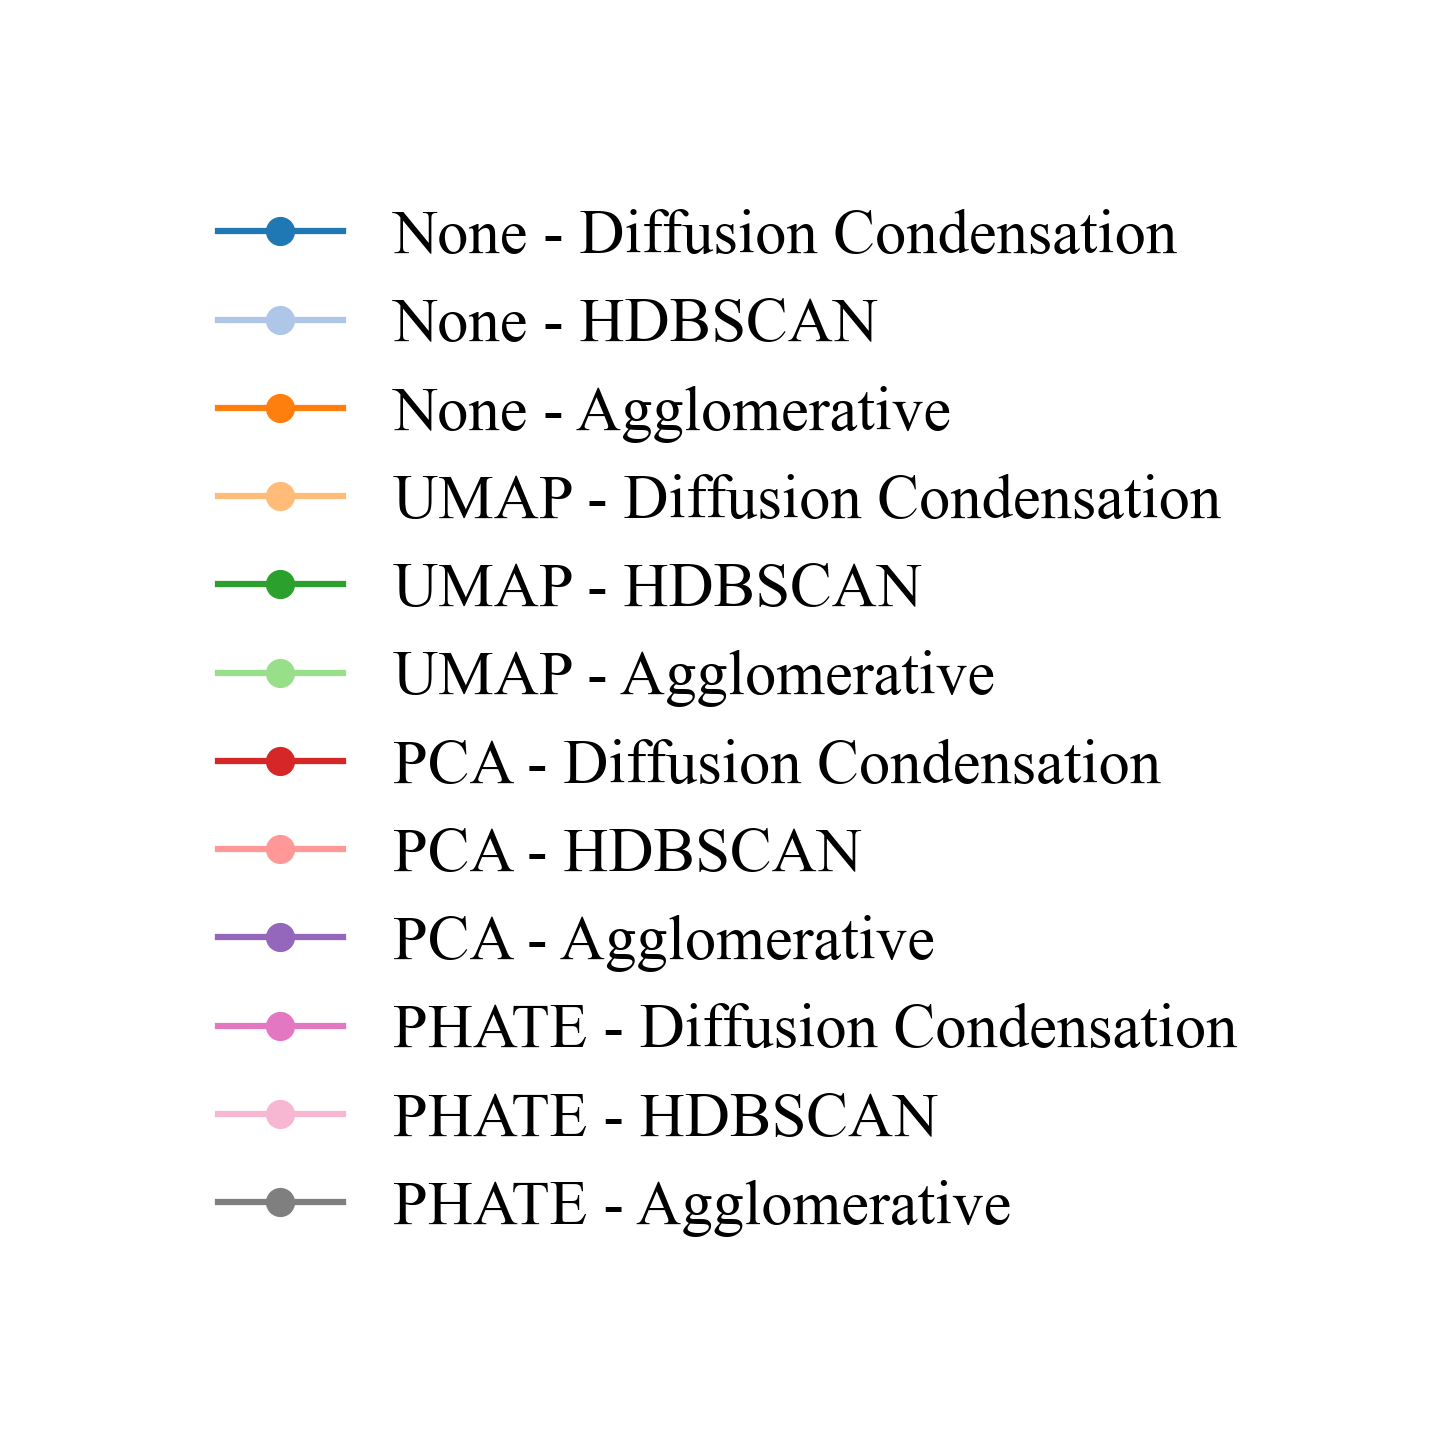
\includegraphics[width=\linewidth]{legend_None_t1.0_maxsub3_depth5_noiseNone_random.png}
    \end{minipage}
    \caption{Line plot of performance at each cluster level averaged across deep and shallow generated datasets. Lower numbers on the x-axis correspond to coarser scales (i.e., fewer clusters). \textit{None} means no dimensionality reduction. Bars represent standard error.}
    \label{fig:ARI-combined}
\end{figure*}